% mainfile: ../../../../master.tex
\subsection{DNA and RNA quantification with NanoDrop\cR ND-1000 Spectrophotometer}
% The part of the label after the colon must match the file name. Otherwise,
% conditional compilation based on task labels does NOT work.
\label{task:20180227_cj1}
\tags{lab,qnt,dna,rna,extr}
\authors{cj}
%\files{}
%\persons{}

\begin{figure}[H] % position of the figure 
    \centering
    \caption{Title of the figure}
    \label{fig:label}
    \begin{subfigure}[b]{0.49\textwidth}
        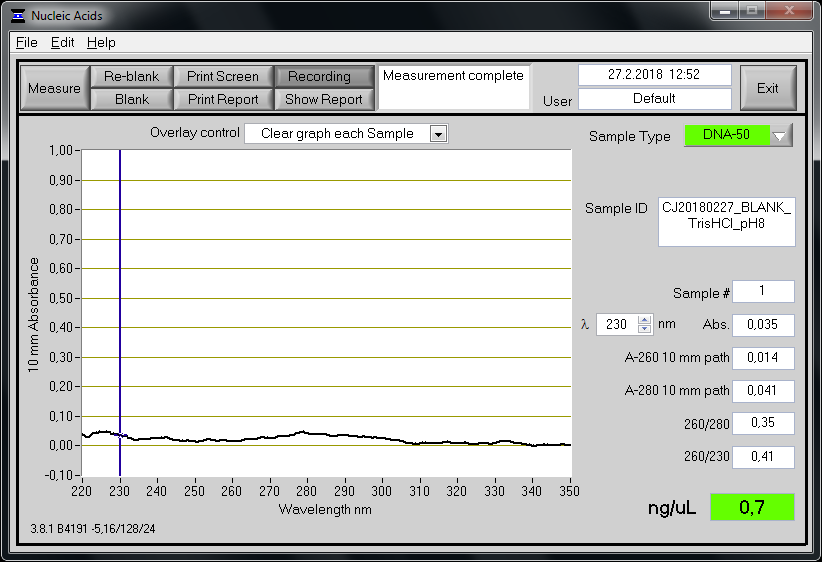
\includegraphics[width=\textwidth]{graphics/screenshots/CJ20180227_BLANK_TrisHCl_pH8.png}
        \caption{Spectrum of the Tris-HCl buffer pH 8 used as Blank}
        \label{sfig:CJ20180227_BLANK_TrisHCl_pH8}
    \end{subfigure}
    ~ 
    \begin{subfigure}[b]{0.49\textwidth}
        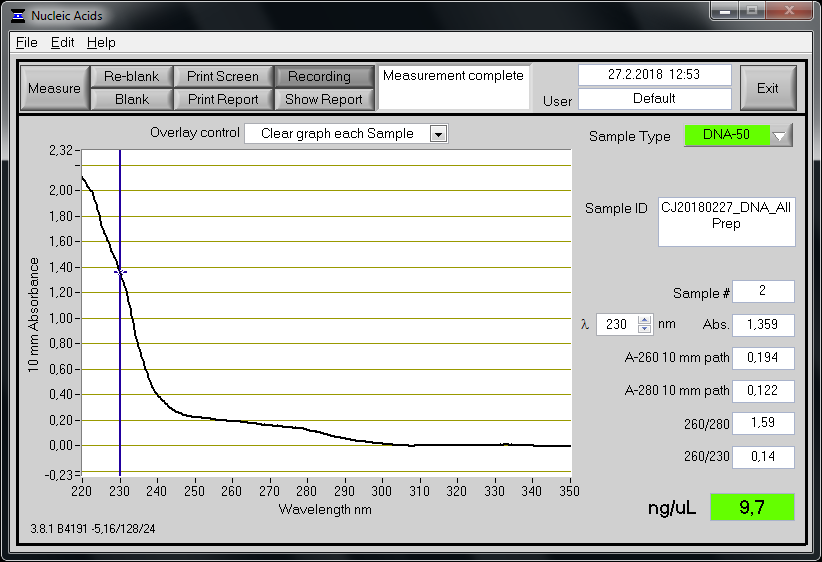
\includegraphics[width=\textwidth]{graphics/screenshots/CJ20180227_DNA_AllPrep.png}
        \caption{Spectrum of the DNA extracted with AllPrep}
        \label{sfig:CJ20180227_DNA_AllPrep}
    \end{subfigure}
    \\
    \begin{subfigure}[b]{0.49\textwidth}
        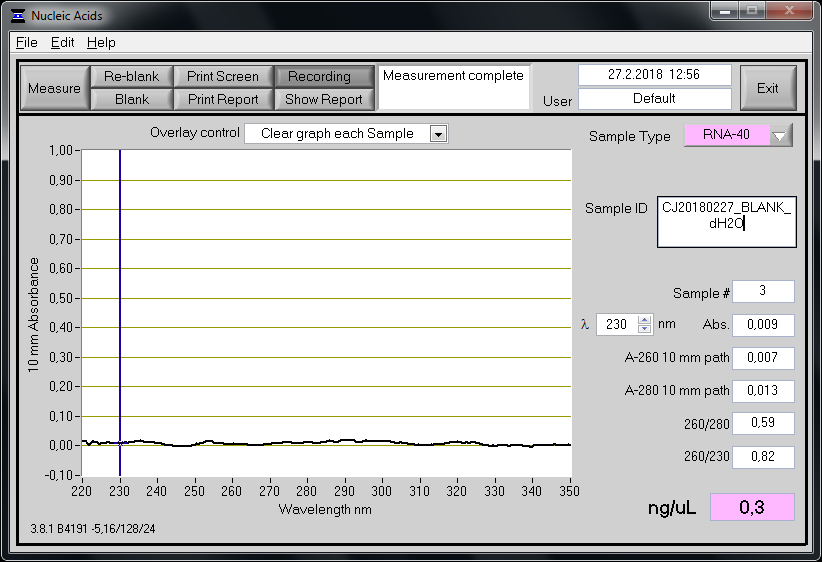
\includegraphics[width=\textwidth]{graphics/screenshots/CJ20180227_BLANK_dH2O.png}
        \caption{Spectrum of the dH2O used as Blank}
        \label{sfig:CJ20180227_BLANK_dH2O}
    \end{subfigure}
    ~ 
    \begin{subfigure}[b]{0.49\textwidth}
        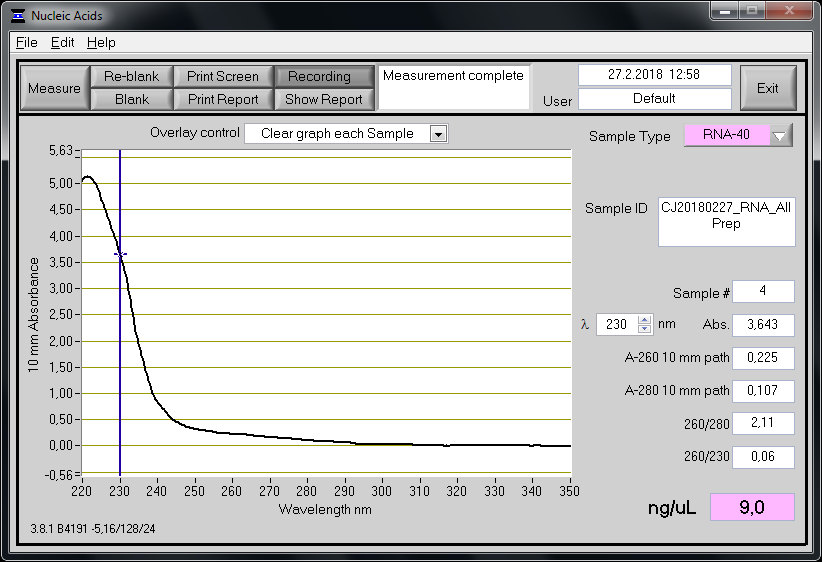
\includegraphics[width=\textwidth]{graphics/screenshots/CJ20180227_RNA_AllPrep.png}
        \caption{Spectrum of the RNA extracted with AllPrep}
        \label{sfig:slabel2}
    \end{subfigure}
\end{figure}